% E.16 等边 △ABC, 内点 P, PA=3, PB=4, PC=5. 由旋转知 ∠APB=150°, 边长²=25+12√3.
% 边长 a=√(25+12√3)≈√45.78≈6.766. △APB 绕 B 顺时针 60° → △CP'B, P→P'. PP'=PB=4, △PP'C: PP'=4,P'C=PA=3,PC=5 → 直角.
% 取 B(0,0), C(6.766,0), A=B+a·(cos60°,sin60°)=(3.383, 5.859)
% P: 满足 PA=3,PB=4,PC=5. 用 |PB|=4 与 |PC|=5: P 在两圆交. (x²+y²=16, (x-6.766)²+y²=25) → -13.532x+45.78=9 → x=2.7152, y²=16-7.37=8.63, y=2.938. 验 PA: √((3.383-2.715)²+(5.859-2.938)²)=√(0.446+8.532)=√8.98≈3.0 ✓
% P' = P 绕 B 顺时针 60°: (x,y) → (x·cos(-60)-y·sin(-60), x·sin(-60)+y·cos(-60)) = (0.5x+√3/2·y, -√3/2·x+0.5y)
% = (0.5·2.715+0.866·2.938, -0.866·2.715+0.5·2.938) = (1.358+2.544, -2.351+1.469) = (3.902, -0.882)
\documentclass[tikz,border=4pt]{standalone}
\usepackage{ctex}
\usepackage{amsmath}
\usetikzlibrary{calc}
\begin{document}
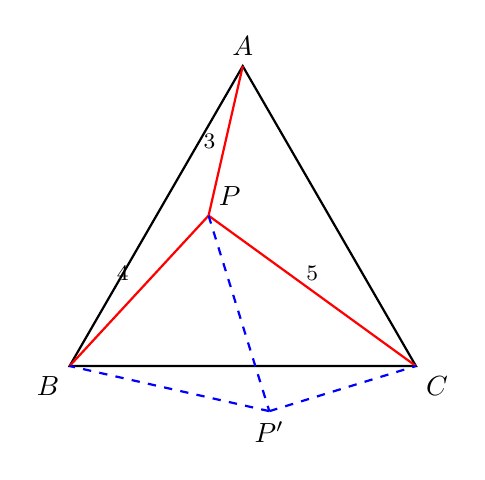
\begin{tikzpicture}[scale=0.65, thick]
  \coordinate (B) at (0,0);
  \coordinate (C) at (6.766,0);
  \coordinate (A) at (3.383, 5.859);
  \coordinate (P) at (2.715, 2.938);
  \coordinate (Pp) at (3.902, -0.882);

  \draw (A)--(B)--(C)--cycle;
  \draw[red, thick] (P)--(A);
  \draw[red, thick] (P)--(B);
  \draw[red, thick] (P)--(C);
  \draw[blue, dashed, thick] (Pp)--(B);
  \draw[blue, dashed, thick] (Pp)--(C);
  \draw[blue, dashed, thick] (P)--(Pp);

  \node[above] at (A) {$A$};
  \node[below left] at (B) {$B$};
  \node[below right] at (C) {$C$};
  \node[above right] at (P) {$P$};
  \node[below] at (Pp) {$P'$};

  \node[font=\footnotesize, left] at ($(P)!0.5!(A)$) {$3$};
  \node[font=\footnotesize, above left] at ($(P)!0.5!(B)$) {$4$};
  \node[font=\footnotesize, above] at ($(P)!0.5!(C)$) {$5$};
\end{tikzpicture}
\end{document}
